\chapter{Metodologia}
Esse capítulo constará, respectivamente, com as informações técnicas referentes aos experimentos (características do computador utilizado, sistema operacional, linguagem de programação adotada, etc), os algoritmos implementados (uma breve explicação de cada um e seus respectivos códigos) e uma explicação de cada cenário analisado nesse trabalho.

\section{Informações técnicas}
Para a realização do trabalho, foi utilizado um notebook com as seguintes características:

\begin{tabular}{| r | l |}
	\hline
	\textbf{Fabricante}   & Acer \\
	\hline
	\textbf{Modelo}       & Aspire 4739 \\
	\hline
	\textbf{Placa-mãe}    & HMA CP (versão 1.08) \\
	\hline
	\textbf{Disco}        & Hitachi HTS54757 (750 GB) \\
	\hline
	\textbf{RAM}          & 8 GB \\
	\hline
	\textbf{Processador}  & Intel Core i5-480M (2.67GHz) \\
	\hline
	\textbf{Gráficos}     & Intel Ironlake Mobile \\
	\hline
	\textbf{Sistema base} & Ubuntu 16.04.2 LTS 64-bit \\
	\hline
\end{tabular}

A linguagem de programação adotada foi \textbf{C++} (\textit{C mais mais} ou \textit{C plus plus}). C++ foi escolhido devido ser considerado uma linguagem poderosa para a resolução de problemas de baixo e alto nível, prezando pela performance rápida, pois cada recursos presente foi criteriosamente projetado para se usado onde performance for uma exigência crítica \cite{meyers1997cpp}.

O compilador usado foi o \textbf{g++}, compilador integrante da \texttt{gcc}\footnote{Originalmente escrito como compilador para o sistema operacional GNU, a \textit{GNU Compiler Collection} é um conjunto de compiladores de diversas linguagens (C, C++, Fortran, Ada, Go, etc) e é distribuído pela \textit{Free Software Foundation} (FSF). Seu site oficial é: \url{https://gcc.gnu.org/}.}. Para automatizar a compilação, fez-se uso de um arquivo Makefile\footnote{O arquivo Makefile define regras de compilação que serão seguidas no projeto. Ele é interpretado pelo programa \textbf{make}. A página oficial é: \url{https://www.gnu.org/software/make/}.}.

O editor de texto usado para escrever os códigos usados no trabalho foi o \textbf{Sublime text}\footnote{Site oficial: \url{https://www.sublimetext.com/}.}.

\section{Algoritmos implementados}
Nessa seção será descrito os algoritmos implementados e análisados, como também será posto seus respectivos códigos usados no projeto. Perceba que todas as funções possuem a mesma assinatura. Isso foi feito para facilitar na implementação dos códigos no projeto.

\subsection{Insertion sort}
O \textit{Insertion sort} funciona da seguinte maneira: você tem como entrada um vetor de elementos, ele irá percorrer índice por índice e a cada iteração pega aquele elemento e o coloca na posição correta, realizando as trocas necessárias com os elementos anteriores para só depois avançar na iteração. Para entender melhor, veja a imagem a seguir:

\begin{figure}[!htb]
	\centering
	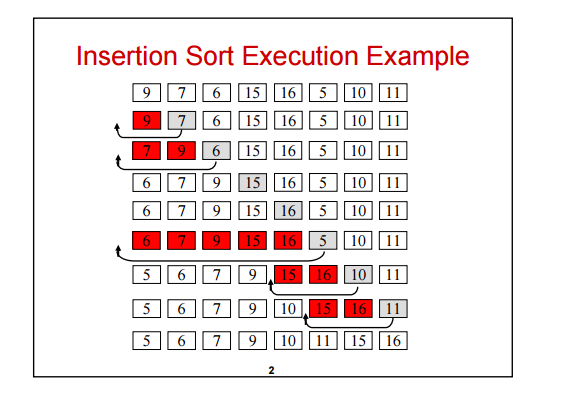
\includegraphics{img/insertion-sort.png}
	\caption{Insertion Sort.}
	\small{Imagem retirada de: \url{http://www.geeksforgeeks.org/insertion-sort/}.}
	\label{insertion-sort}
\end{figure}

Suas informações referentes a complexidade e estabilidade são:

\begin{table}[H]
 \centering
	\begin{tabular}{| r | l |}
		\hline
		\textbf{Complexidade pior caso}   & $O(n^{2})$ \\
		\hline
		\textbf{Complexidade caso médio}  & $O(n^{2})$ \\
		\hline
		\textbf{Complexidade melhor caso} & $O(n)$ \\
		\hline
		\textbf{Estabilidade}             & Estável \\
		\hline
	\end{tabular}
	\caption{Complexidade e estabilidade do Insertion Sort.}
	\label{t_insertion_sort}
\end{table}

No código a seguir, passamos como argumento o vetor que queremos ordenar. Ignoramos os outros dois parâmetros (\texttt{\_left} e \texttt{\_right}), pois eles foram colocados para apenas termos as mesmas assinaturas que as outras funções do projeto.

\lstinputlisting{codes/insertion_sort.cpp}

\subsection{Selection sort}
O \textit{Selection sort} funciona da seguinte maneira: você tem como entrada um vetor de elementos, ele irá percorrer todo o vetor atrás do menor elemento. Após percorrido, irá trocar a posição do elemento de menor valor com a posição da iteração. Assim, a cada ciclo ele garante que os elementos da posição inicial até $i-1$ ($i$ = iteração) já estejam ordenados. Para entender melhor, veja a imagem a seguir:

\begin{figure}[!htb]
	\centering
	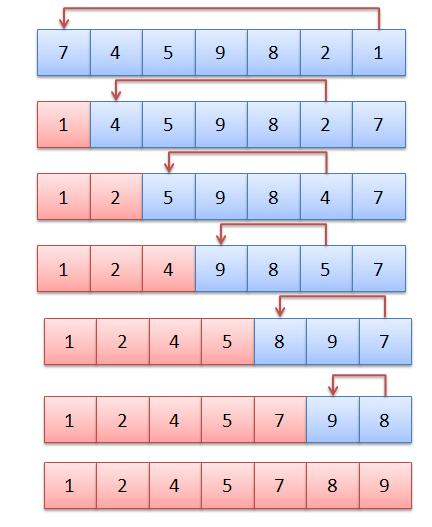
\includegraphics{img/selection-sort.jpg}
	\caption{Selection Sort.}
	\small{Imagem retirada de: \url{http://nerds-attack.blogspot.com.br/2012/09/estrutura-dados-selection-sort.html}.}
	\label{selection-sort}
\end{figure}

Suas informações referentes a complexidade são:

\begin{table}[H]
 \centering
	\begin{tabular}{| r | l |}
		\hline
		\textbf{Complexidade pior caso}   & $O(n^{2})$ \\
		\hline
		\textbf{Complexidade caso médio}  & $O(n^{2})$ \\
		\hline
		\textbf{Complexidade melhor caso} & $O(n^{2})$ \\
		\hline
	\end{tabular}
	\caption{Complexidade do Selection Sort.}
	\label{t_selection_sort}
\end{table}

No código a seguir, passamos como argumento o vetor que queremos ordenar. Ignoramos os outros dois parâmetros (\texttt{\_left} e \texttt{\_right}), pois eles foram colocados para apenas termos as mesmas assinaturas que as outras funções do projeto.

\lstinputlisting{codes/selection_sort.cpp}

\subsection{Bubble sort}
O \textit{Bubble sort} funciona da seguinte maneira: você tem como entrada um vetor de elementos, a cada iteração ele irá realizar trocas do elemento atual com os seus seguintes até encontrar a posição ideal do elemento. Para entender melhor, veja a imagem a seguir:

\begin{figure}[!htb]
	\centering
	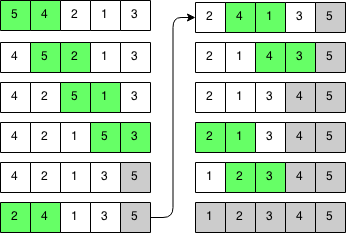
\includegraphics{img/bubble-sort.png}
	\caption{Bubble Sort.}
	\small{Imagem retirada de: \url{http://www.coisadeprogramador.com.br/algoritmos-ordenacao-bubble-sort/}.}
	\label{bubble-sort}
\end{figure}

Suas informações referentes a complexidade são:

\begin{table}[H]
 \centering
	\begin{tabular}{| r | l |}
		\hline
		\textbf{Complexidade pior caso}   & $O(n^{2})$ \\
		\hline
		\textbf{Complexidade caso médio}  & $O(n^{2})$ \\
		\hline
		\textbf{Complexidade melhor caso} & $O(n)$ \\
		\hline
	\end{tabular}
	\caption{Complexidade do Bubble Sort.}
	\label{t_bubble_sort}
\end{table}

No código a seguir, passamos como argumento o vetor que queremos ordenar. Ignoramos os outros dois parâmetros (\texttt{\_left} e \texttt{\_right}), pois eles foram colocados para apenas termos as mesmas assinaturas que as outras funções do projeto.

\lstinputlisting{codes/bubble_sort.cpp}

\subsection{Shell sort}
O \textit{Shell sort} é uma extensão do algoritmo \textit{Insertion sort}. Diferente do \textit{Selection sort} que só permite realizar trocas de elementos adjacentes, o \textit{Shell sort} permite trocas de elementos distantes um do outro. Ele funciona da seguinte maneira: você tem como entrada um vetor de elementos, usamos o tamanho desse vetor para decidir qual será a distância inicial entre os elementos que serão trocados. Após cada iteração, dividiremos a distância e assim sucessivamente até atingirmos a troca de elementos adjacentes. Para entender melhor, veja a imagem a seguir:

\begin{figure}[!htb]
	\centering
	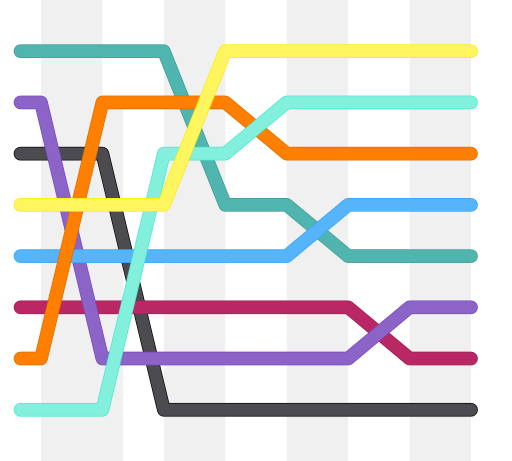
\includegraphics{img/shell-sort.png}
	\caption{Shell Sort.}
	\small{Imagem retirada de: \url{https://pt.wikipedia.org/wiki/Shell_sort}.}
	\label{shell-sort}
\end{figure}

A sua análise contêm alguns problemas matemáticos muito difíceis, por causa disso, a sua complexidade ainda não é totalmente conhecida. Suas informações referentes a complexidade até então conhecidas são:

\begin{table}[H]
 \centering
	\begin{tabular}{| r | l |}
		\hline
		\textbf{Complexidade pior caso}   & $O(nlog_{2}n)$ (melhor conhecida) \\
		\hline
		\textbf{Complexidade caso médio}  & depende da sequência da distância \\
		\hline
		\textbf{Complexidade melhor caso} & $O(n)$ \\
		\hline
	\end{tabular}
	\caption{Complexidade do Shell Sort.}
	\label{t_shell_sort}
\end{table}

No código a seguir, passamos como argumento o vetor que queremos ordenar. Ignoramos os outros dois parâmetros (\texttt{\_left} e \texttt{\_right}), pois eles foram colocados para apenas termos as mesmas assinaturas que as outras funções do projeto. Perceba que dividimos a variável `gap' em $2.2$, isso ocorre porque se a divisão der, por exemplo, $2.72727$, pegaremos apenas o valor inteiro, ou seja: $2$. Assim não teremos problemas na execução do algoritmo.

\lstinputlisting{codes/shell_sort.cpp}

\subsection{Quicksort}
\subsection{Merge sort}
\subsection{Radix sort (LSD)}

\subsection{Visão geral}
\begin{table}[H]
 \centering
	\begin{tabular}{| r | p{2.5cm} | p{2.5cm} | p{2.5cm} |}
		\hline
		\multirow{2}{*}{textbf{Algoritmo}} & \multicolumn{3}{c|}{\textbf{Complexidade}} \\
		 & Melhor caso   & Caso médio & Pior caso \\
		\hline
		Insertion sort   & $O(n)$          & $O(n^{2})$                        & $O(n^{2})$ \\
		\hline
		Selection sort   & $O(n^{2})$      & $O(n^{2})$                        & $O(n^{2})$ \\
		\hline
		Bubble sort      & $O(n)$          & $O(n^{2})$                        & $O(n^{2})$ \\
		\hline
		Shell sort       & $O(n)$          & Depende da sequência da distância & $O(nlog_{2}n)$ (melhor conhecida) \\
		\hline
		Quicksort        & $O(nlog_{2}n)$  & $O(nlog_{2}n)$                    & $O(n^{2})$ \\
		\hline
		Merge sort       & $\theta(nlogn)$ & $\theta(nlogn)$                   & $\theta(nlogn)$ \\
		\hline
		Radix sort (LSD) &                 &                                   & $\theta(nk)$ \\
		\hline
	\end{tabular}
	\caption{Complexidade e estabilidade do Insertion Sort}
	\label{t_insertion_sort}
\end{table}

\section{Cenários}
No projeto foi-se aplicado os algoritmos anteriormente apresentados em um total de 3 cenários distintos. Informações sobre esses cenários podem ser vistos logo a seguir.

\subsection{Arranjos com elementos aleatórios}


\subsection{Arranjos com elementos não decrescentes}
\subsection{Arranjos com elementos não crescentes}